\documentclass[12pt, a4paper, openany]{book}
\usepackage{../../generalStyle}
\graphicspath{ {./img} }

\lstset{
  language=SQL,
  basicstyle=\ttfamily,
  keywordstyle=\color{blue},
  stringstyle=\color{red},
  commentstyle=\color{green},
  morecomment=[l][\color{magenta}]{\#}
}

\begin{document}

\title{Basi di dati}
\author{
    Elia Ronchetti\\
	\small{\href{https://t.me/ulerich}{@ulerich}}
}
\date{Marzo 2022}

\maketitle
\tableofcontents

\chapter*{Introduzione}

Questi appunti di Analisi Matematica sono stati fatti con l'obiettivo di riassumere tutti (o quasi) gli argomenti utili per l'esame di Analisi Matematica del corso di Informatica dell'Università degli Studi di Milano Bicocca.
\\Come fonte ho utilizzato:
\begin{itemize}
	\item Appunti di altri studenti.
	\item Libro "Analisi Uno, teoria ed esercizi" di Giuseppe De Marco (terza edizione).
	\item Esercitazioni in aula della professoressa Susanna Caimi.
\end{itemize}
\section*{Il Corso}
Come già detto, questi appunti sono in funzione del corso di Analisi Matematica di UNIMIB, a.a. 2021/22, insegnato dalla Professoressa Pini.
\subsection*{Programma del corso}
\begin{enumerate}
	\item Numeri Reali
	      \begin{enumerate}
		      \item Funzioni elementari
		      \item Generalità sulle funzioni
		      \item Funzioni reali di una variabile
	      \end{enumerate}
	\item Successioni
	      \begin{enumerate}
		      \item Limiti di successioni reali
		      \item Principio di Induzione
		      \item Limiti notevoli
	      \end{enumerate}
	\item Limiti e continuità
	      \begin{enumerate}
		      \item Limiti di Funzioni
		      \item Limiti notevoli
		      \item Funzioni continue
		      \item Proprietà globali delle funzioni continue
	      \end{enumerate}
	\item Calcoli differenziale
	      \begin{enumerate}
		      \item Derivate di una funzione
		      \item Proprietà delle funzioni derivabili
		      \item Funzioni convesse e concave
		      \item Formula di Taylor
		      \item Grafici di funzioni
	      \end{enumerate}
	\item Calcolo integrale
	      \begin{enumerate}
		      \item Funzioni integrabili secondo Rienmann
		      \item Teorema fondamentale del calcolo e integrali indefiniti
		      \item Metodi d'integrazione
	      \end{enumerate}
	\item Serie numeriche
	      \begin{enumerate}
		      \item Serie, convergenza, convergenza assoluta
		      \item Serie a termini positivi
		      \item Serie a termini di segno variabile
	      \end{enumerate}
\end{enumerate}

\subsection*{Prerequisiti}
\begin{itemize}
	\item \emph{Algebra elementare}: Calcolo letterale, equazioni e disequazioni di primo e secondo grado
	\item \emph{Trigonometria elementare}
	\item \emph{Esponenziali e logaritmi}
\end{itemize}

\chapter{ER modeling}
\section{Entità}
Definita come sostantivo al singolare (es. studente, classe, docente, ecc.)
A livello estensionale un'entità è costituira da un insieme di oggetti 
che sono chiamati le sue istanze.
\chapter{Modello Relazionale}
\label{sec:Modello_relazionale}
Un modello dei dati è un insieme di concetti per organizzare i dati e 
descriverne la struttura.
Componente fondamentale di ogni modello sono i meccanismi di strutturazione 
(analogi ai costruttori di tipo).
\\ Ogni modello dei dati prevede alcuni costruttori che permettono di definire nuovi
tipi sull abase di tipi predefiniti (elementari).
\\ Il \textbf{modello relazionale} è il modello di dati più diffuso.
\section{Introduzione al modello relazionale e cenni storici}
Il modello relazionale permette di definire tipi per mezzo del costruttore \textbf{relazione}
 che permette di organizzare i dati in insiemi di recordo a \textbf{struttura fissa}.
 \\ Una \textbf{relazione} è spesso rappresentata da una tabella, dove:
 \begin{itemize}
    \item Le righe rappresentano specifici record (istanze)
    \item Le colonne corrispondono ai campi dei record
 \end{itemize}
 L'ordine di righe e colonne è sostanzialmente irrilevante.
 La tabella è il livello logico di cui parlavamo inizialmente (schema DBMS, divisione
 livello fisico e logico). Ribadiamo che il livello logico è indipendente da quello
 fisico infatti una tabella è utilizzata nello stesso modo qualunque sia la sua realizzazione
 fisica. In questo corso vedremo solo il livello logico.
 \subsection{I modelli logici dei dati}
 Tradizionalmente ci sono tre modelli logici:
 \begin{itemize}
    \item Gerarchico - Organizzazione ad albero
    \item Reticolare - Organizzazione a grafo
    \item Relazionale - Organizzazione a tabella
 \end{itemize}
 Poi ci sono altri modelli più recenti (e meno diffusi)
 \begin{itemize}
    \item a oggetti
    \item XML
    \item NoSQL - Basato su documenti
 \end{itemize}
 \subsection{Il modello relazionale}
 Proposto da E.F. Codd nel 1970 per favorire l'indipendenza dei dati, è
 diventato disponibile in DBMS reali nel 1981.
 \\ \'E basato sul concetto matematico di relazione a livello formale (con una variante),
 mentre concettualmente è basato su tabelle.
 \\ Essendo uno schema logico definisce come sono organizzati i dati e non come
 sono memorizzati e gestiti dal sistema informatico.
 \subsection{Il termine relazione in 3 accezioni}
 \begin{enumerate}
    \item Relazione matematica - come nella teoria degli insiemi
    \item Relazione - secondo il modello relazionale dei dati
    \item Relazione (dall'inglese relationship) che rappresenta una classe di fatti,
    nel modello Entity-Relationship, tradotto anche con associazione e correlazione
 \end{enumerate}
 \section{Modello relazionale - definizione formale}
 Dati due insiemi $D_1, \,D_2$ (Estendibile a n insiemi distinti o non), si definisce
 \textbf{prodotto cartesiano} $D_1 x D_2$ come l'insieme di tutte le possibili coppie
 ordinate $(v_1, v_2)$ tali che $v1 \in D_1$ e $v_2 \in D_2$.
 \paragraph*{Esempio} $A=\{1,2,4\}$ e $B=\{a,b\}$ il prodotto cartesiano $AxB$ è
 composto da $\{(1,a), (1,b), (2,a), (2,b), (3,a), (3,b)\}$, cioè le sei coppie ordinate
 (il primo da A e il secondo da B) senza ripetizioni.
 \\ Il prodotto cartesiano rappresenta l'insieme di tutte le n-uple ordinate,
 mentre la \textbf{relazione matematica} rappresentare un sottoinsieme del prodotto
 cartesiamo fra n insiemi. Gli insiemi di partenza sono chiamati \textbf{domini},
 mentre il numero delle componenti del prodotto (n) è detto grado della relazione, 
 il numero di n-uple della relazione è la \textbf{cardinalità} della relazione.
 
\chapter{Progettazione Concettuale}
\chapter{Algebra Relazionale}
Nell ebasi di dati relazionali esistono 2 tipi di linguaggi di interrogazione
\begin{itemize}
    \item Procedurali - Specificano le modalità di generazione del risultato - Come
    \item Dichiarativi - Specificano le proprietà del risultato - Che cosa
\end{itemize}
L'algebra relazionale è procedurale, mentre SQL è parzialmente dichiarativo.\\
L'algebra relazionale è composta da un insieme di operatori che possono essere
utilizzati su relazioni per produrre relazioni. Possono essere composti dando
luogo a espressioni algebriche di complessità arbitraria.\\
\section{Operatori dell'algebra relazionale}
\paragraph*{Unarie}
\begin{itemize}
    \item Ridenominazione
    \item Selezione
    \item Proiezione
\end{itemize}
\paragraph*{Binarie}
\begin{itemize}
    \item Unione, Intersezione, Differenza (Operatori insiemistici)
    \item Join (Join naturale, Prodotto cartesiano, Theta-join)
\end{itemize}
\section{Operatori insiemistici}
Le relazioni sono insiemi e quindi è possibile applicare gli operatori insiemistici,
è fondamentale sapere che è possibile applicare queste operazioni \textbf{solo a relazioni
    definite sugli stessi attributi}.
\subsection*{Unione}
L'unione di due relazioni $r_1$ e $r_2$ è la relazione che contiene le tuple
che appartengono ad $r_1$ oppure ad $r_2$, oppure ad entrambe.\\
L'unione è commutativa e associativa.
\subsection*{Intersezione}
L'intersezione di due relazioni $r_1$ e $r_2$ è la relazione che contiene le tuple
che appartengono sia a $r_1$ che a $r_2$.\\
L'intersezione è commutativa e associativa ed è inoltre esprimibile per mezzo della
differenza:
\begin{equation*}
    r(X) = r_1(X) \cap r_2(X) = r_1(X) - (r_1(X) - r_2(X))
\end{equation*}
\subsection*{Differenza}
La differenze di due relazioni $r_1(X)$ e $r_2(X)$ definite su un insieme di attributi
X è la relazione $r(X) = r_1(X) - r_2(X)$ che contiene le tuple che appartengono a $r_1(X)$, ma
non a $r_2(X)$.\\
La differenza NON è commutativa.\\
\subsection*{Operatori insiemistici e valori nulli}
Gli operatori insiemistici sono definiti anche per relazioni che contengono valori nulli.\\
\section{Operatorri unari}
\subsection{Operatore di ridenominazione}
Per poter applicare operazioni insiemistiche come unione, intersezione, differenza a relazioni
su attributi in parte diversi è necessario ridenominare attributi, in modo da uniformare
i nomi. Questo viene fatto dall'operatore ridenominazione.\\
Si tratta di un operatore monadico (cioè un solo argomento) che modifica lo schema lasciando
inalterata l'istanza dell'operando. Cambia quindi il nome dell'attributo, ma non il valore.
\paragraph*{Sintassi} Si indica con $\rho_{y \leftarrow x}(r)$ o 
$\text{REN}_{y \leftarrow x}(r)$, dove x è
il nome originale dell'attributo, mentre y è quello nuovo. L'operatore è sempre seguito dal
nome della relazione che stiamo considerando.\\
\'E possibile rinominare più attributi, in questo caso è importante l'ordine degli attributi
dato che la sintassi sarà la seguente:
\begin{equation*}
    \rho_{y1, y_2 \leftarrow x_1, x_2}(r)
\end{equation*}
\paragraph*{Esempio}
\begin{tabular}{|c|c|c|}
    \hline
    \textbf{Padre} & \textbf{Figlio} \\
    \hline
    Adamo          & Abele           \\
    \hline
    Adamo          & Caino           \\
    \hline
\end{tabular}
$\text{REN}_{\text{Genitore}\leftarrow\text{Padre}}(\text{Paternità})$
\begin{tabular}{|c|c|c|}
    \hline
    \textbf{Genitore} & \textbf{Figlio} \\
    \hline
    Adamo          & Abele           \\
    \hline
    Adamo          & Caino           \\
    \hline
\end{tabular}\\
Questa operazione è fondamentale per poter effettuare operazioni insiemistiche tra
relazioni con attributi diversi, in questo modo possiamo uniformare i nomi degli attributi.
\subsection{Selezione}
Permette di selezionare un sottoinsieme delle ennuple, producendo un risultato che:
\begin{itemize}
    \item Ha lo stesso schema dell'operando
    \item Contiene un sottoinsieme delle ennuple dell'operando
    \item Contene le ennuple che soddisfano una condizione espressa dall'operatore
\end{itemize}
\paragraph*{Sintassi} $\sigma_{\text{condizione}}(r) \\$
\paragraph*{Sintassi alternativa}$\text{SEL}_{\text{condizione}}(r)$
Data una relazione r(X) è una formula ottenuta combinando con i connettivi OR, AND e NOT
condizioni atomiche del tipo:
\begin{itemize}
    \item CONFR è un operatore di confronto ($=, <, >, \geq, \leq$)
    \item A e B sono attributi in X sui cui valori CONFR abbia senso
    \item c'è una costante per cui il confronto CONFR sia definito
\end{itemize}
Il risultato contiene le ennuple dell'operando che soddisfano la condizione (cioè su cui
la condizione è vera).
\paragraph*{Esempi} Impiegati che:
\begin{itemize}
    \item Guadagnano più di 50 - STIPENDIO $>$ 50
    \item Guadagnano più di 50 e lavorano a Milano - STIPENDIO $>$ 50 AND FILIALE = 'Milano'
    \item Hanno un cognome uguale al nome della filiale presso cui lavorano - COGNOME = FILIALE
\end{itemize}
Tradotto in Query in Algebra Realzionale: $\text{SEL}_{\text{Stipendio} > 50}(\text{Impiegati})$,
lo stesso per le altre query, la parte scritta andrà sostituita nella parte condizione (sotto il SEL).
\subsection*{Selezione con valori nulli}
La condizione atomica è vera solo per valori non nulli.\\
Se per esempio effettuo una SEL su una tabella con valori nulli, e la condizione seleziona
tutti gli attributi (es. $\text{SEL}_\text{Età}>30 \cup \text{SEL}_\text{Età}\leq30$) 
il risultato sarà una tabella diversa da quella di partenza, perchè le condizioni atomiche
vengono valutate separatamente e i valori nulli non sono valori che possiamo confrontare con un numero
dato che rappresentano un valore di verità intermedio tra vero e falso. Anche inserendo tutto in una
unica SEL il risultato sarebbe il medesimo, quindi senza valori nulli. \\
Per questo esistono gli operatori \textbf{IS NULL e IS NOT NULL}. Per avere la tabella iniziale
per l'esempio Persone basterebbe quindi unire la precedente SEL con la seguente: 
$\text{SEL}_\text{Età IS NULL}(\text{Persone})$. In questo modo otteniamo la
stessa relazione di partenza dato che consideriamo anche i valori NULL.

\section{Proiezione}
Si occupa di selezionare solo alcune delle colonne della tabella presa in considerazione. \\
Per fare un confronto con il SEL:
\begin{itemize}
    \item SEL è un operatore ortogonale di decomposizione orizzontale, infatti
    riduce il numero di righe
    \item PROJ è un operatore ortogonale di decomposizione verticale, infatti
    riduce il numero di colonne
\end{itemize}
Si tratta anche in questo caso di un operatore monadico.
\paragraph*{Sintassi} $\text{PROJ}_{\text{lista di attributi}}(\text{Operando})$, il risultato
conterrà le ennuple dell'perando ristrette ai soli attributi nella ListaAttributi.
\subsection*{Proiezione e Valori Null}
Proiezione, unione e differenza continuano a comportarsi usualmente quindi due tuple sono uguali
anche se ci sono dei NULL. \\
Dato che una relazione è un insieme e un insieme non ha elementi uguali il risultato
della PROJ non conterrà ennuple uguali, esse saranno scartate.
\subsection*{Cardinalità delle proiezioni}La cardinalità di una relazione è il numero delle sue ennuple e
si indica con $|R|$.\\
Una proiezione:
\begin{itemize}
    \item Contiene al più tante ennuple quante l'operando
    \item Può anche contenerne di meno (come spiegato in precedenza)
\end{itemize}
Vale la proprietà che \textbf{se X è una superchiave di R, allora  $\text{PROJ}_X(R)$} contiene
esattamente tante ennuple quante R.\\
Per la definizione di superchiave ogni superchiave compare una sola volta nella relazione.\\
\subsection*{Selezione e Proiezione}
Combinando selezione e proiezione possiamo estrarre interessanti informazioni da una realzione
\paragraph*{Esempio}
\begin{table}[]
    \begin{tabular}{|l|l|l|l|}
    \hline
    Matricola & Cognome & Filiale & Stipendio \\ \hline
    7309      & Neri    & Napoli  & 55        \\ \hline
    5998      & Neri    & Milano  & 64        \\ \hline
    9553      & Rossi   & Roma    & 44        \\ \hline
    5698      & Rossi   & Roma    & 64        \\ \hline
    \end{tabular}
\end{table}
Ci viene richiesto matricola e cognome degli impiegati che guadagnano più di 50:
\paragraph*{Soluzione}
\begin{equation*}
    \text{PROJ}_{\text{Matricola, Cognome}}(\text{SEL}_{\text{Stipendio} > 50}(\text{Impiegati}))
\end{equation*}
Inserisco quindi come argomento della PROJ la SEL delle tuple richieste. Combinando questi due
operatori posso estrarre informazioni da una relazione. Non possiamo però correlare,
mettere insieme informazioni presenti in relazioni diverse, per questo esiste il JOIN.

\section{Join}
Il Join è senz'altro l'operatore più interessante dell'algebra relazionale dato che permette
di correlare, mettere insieme, integrare dati che si trovano in relazioni diverse. Ci sono
diversi tipi di Join, partiamo da quello naturale.
\subsection*{Join naturale}
Operatore binario (generalizzazione), produce un risultato sull'unione degli attributi
degli operandi con ennuple costruite ciascuna a partire da una ennupla di ognuno degli operandi.
\paragraph*{Sintassi} Date due relazioni $R_1(X_1)$ e $R_2(X_2)$, $R_1 \text{JOIN} R_2$ è una
relazione su $X_1, X_2$. Contribuiscono quindi le ennuple che hanno gli stessi valori negli attributi
comuni. Quando ogni ennupla contribuisce al risultato si dice \textbf{Join completo}.\\
Un Join è non completo quando ci sono attributi sulle due relazioni che non corrispondono fra di loro. Se
nessun attributo trova una corrispondenza si ottiene un Join vuoto.\\
Il join si indica anche con $\bowtie$.
\subsection*{Cardinalità del Join}
\begin{enumerate}
    \item Il Join di $R_1$ e $R_2$ contiene un numero di ennuple compreso fra zero e il prodotto di $|R_1|$
    e $|R_2|$
    \item Se il Join coinvolge una chiave di $R_2$ allora il numero di ennuple è compreso fra zero e $|R_1|$.
    \item Se B è chiave in $R_2$ ed esiste vincolo di integrità referenziale fra
    B (in $R_1$) e $R_2$, allora il numero di ennuple è uguale a $|R_1|$\\ $|R_1 \,\text{JOIN}\, R_2| = |R_1|$
\end{enumerate}
Il Join è commutativo e associativo.\\
Il Join naturale non combina due tuple se queste hanno entrambe valore nullo su un attributo in
comune (e valori uguali sugli eventuali altri attributi comuni).
\subsection*{Proprietà del Join}
In assenza di valor nulli l'intersezione di $r_1$ e $r_2$ si può esprimere
\begin{itemize}
    \item mediante il join naturale $r_1 \cap r_2 = r_1 \text{JOIN} r_2$ oppure
    \item sfruttando l'uguaglianza $r_1 \cap r_2 = r_1 - (r_1 - r_2)$
\end{itemize}
In presenza di valori nulli, dalle definizioni date si ha che:
\begin{itemize}
    \item nel primo caso il risultato non contiene tuple con valori nulli 
    \item nel secondo caso, viceversa, tali tuple compaiono nel risultato
\end{itemize}
Nel Join naturale le ennuple che non contribuiscono al risultato vengono tagliate fuori, per
questo viene utilizzato il JOIN esterno.
\subsection*{Join esterno}
Il Join esterno estende, con valori nulli, le ennuple che verrebbero escluse da un join del tipo
precedente (interno). Esiste in tre versioni:
\begin{itemize}
    \item Sinistro $=\bowtie$
    \item Destro $\bowtie=$
    \item Completo $=\bowtie=$
\end{itemize}
\paragraph*{Sinistro $\rightarrow$ LEFT} mantiene tutte le ennuple del primo operando, estenendole
con valori nulli, se necessario.
\paragraph*{Destro $\rightarrow$ RIGHT} mantiene tutte le ennuple del secondo operando, estenendole
con valori nulli se necessario.
\paragraph*{Completo $\rightarrow$ FULL} mantiene tutte le ennuple di entrambi gli operandi
estendendole con valori nulli se necessario.
\subsection*{Prodotto Cartesiano}
Un Join naturale su relazioni che non hanno attributi in comune restituisce un'istanza di 
relazione il cui schema contiene tutti i campi di R (nell'ordine originale) seguiti da tutti
i campi di S (nell'ordine originale). Contiene sempre un numero di ennuple pari al prodotto delle
cardinalità degli operandi (le ennuple sono tutte combinabili).\\
Il prodotto cartesiano ha senso solo se seguito da selezione (dato che produce dati non reali associando
anche tuple tra loro sconnesse a livello semantico). Questa operazione viene chiamata \textbf{theta-join}.
\subsection*{Theta-join}
L'operazione Theta-join viene indicata con $R_1 \,\, \text{JOIN}_{\text{Condizione}}R_2$.\\
La condizione C è spesso una congiunzione AND di atomi di confronto $A_1 \theta A_2$ dove $\theta$ è un
operatore di confronto ($>$, $<$, $=$, $\leq$, $\geq$, $\neq$).\\
Se l'operatore è sempre l'uguaglianza (=) allora si parla di equi-join.\\
\subsection*{Join naturale e Theta-join}
Così come è stato definito, il theta-join richiede in ingresso relazioni con schemi disgiunti,
mentre in diversi libri di testo, lavori scientifici e anche nei DBMS viceversa il theta-join 
accetta relazioni con schemi arbitrati e prende il posto del join naturale, ossia tutti i predicati
del join vengono esplicitati. In questo caso per garantire l'univocità degli attributi nello schema
risultato è necessario ridenominare gli attributi sovrapposti in una delle relazioni o adottare
dei trucchi.\\
Il join naturale utilizza implicitamente i nomi degli attributi per stabilire la condizione,
l'equijoin li indica esplicitamente. I DBMS tipicamente non permettono il join naturale
(solo ultime versioni di SQL lo permettono), però possiamo simularlo per mezzo di altri operatori.
\subsection*{Join e Intersezione}
Quando le due relazioni hanno lo stesso schema ($X_1 = X_2$) allora due tuple fanno match
se e solo se hanno lo stesso valore per tutti gli attributi, ovvero sono identiche, per cui
se $X_1 = X_2$ il join naturale equivale all'intersezione delle due relazioni.
\subsection*{Join e ridenominazione}
Per eseguire il Join di una relazione con se stessa in modo significativo bisogna usare la
ridenominazione.\\ $r(X) \,\, \text{JOIN} \,\,r(X) = r(X)$.\\

\section{Interrogazioni in algebra relazionale}
Dato uno schema R di base di dati, una interrogazione è una funzione che per ogni istanza r di R
produce una relazione su un dato insieme di attributi X.\\
\'E importante definire una metodologia per effettuare le Query per poter trasformare richieste verbali 
in algebra relazionale.
\paragraph*{Metodologia}
\begin{enumerate}
    \item Individua le relazioni coinvolte nella specifica dell'interrogazione, attraverso gli attributi citati e le
    condizioni
    \item Individua i tipi di operazioni necessarie
    \item Individua un possibile ordinamento delle operazioni che porta ad ottenere il risultato
    richiesto
\end{enumerate}
Se si hanno le tabelle sott'occhio è una buona idea effettuare l'interrogazione visivamente
per un solo attributo.\\
L'ordine delle operazioni è importante! Scambiando l'ordine di alcune operazioni potremmo ottenere
espressioni non funzionanti.\\
Esercitarsi rifacendo e capendo le query delle slide è un ottimo allenamento per assimilare
questi concetti.\\
In algebra relazionale non sono previsti i quantificatori universali, manca per esempio l'equivalente di
tutti (simbolo $*$ in SQL), in questi
casi è necessario rivedere la query e riformularla in modo tale da poterla esprimere in algebra relazionale, 
per esempio
esprimendo "tutti guadagnano più di n" come "almeno uno guadagna meno di n, oppure n", esprimendo
così l'operazione tramite differenza insiemistica.
\section{Le viste}
Si tratta di una relazione temporanea, paragonabile a una variabile definita a run time, che alla fine della
query non esiste più. Possono risultare molto comode per salvare risultati intermedi che poi andremo
a riutilizzare anche per altre query, in questo modo non dovremo più ricalcolare qulla query.
\paragraph*{Sintassi} NomeVista = Query
\section{Plus teorici}
\subsection{Rappresentazione delle espressioni tramite alberi}
Ogni espressione dell'algebra relazionale può essere rappresentata tramite un albero, in questo modo
rappresentiamo l'ordine di valutazione degli operatori. Ogni operatore corrisponde
ad un nodo, quindi gli operaetori unari hanno solo un ramo in ingrasso e uno in uscita, mentre
quelli binari hanno 2 rami in entrata e 1 in uscita, la radice è in alto.\\
\subsection{Equivalenza di espressioni}
Due espressioni sono equivalenti se producono lo stesso risultato.
\begin{itemize}
    \item Possono essere assolute se non dipendono dallo schema
    \item Oppure possono dipendere dallo schema
\end{itemize}
I risultati di due Query equivalenti sono sempre equivalenti, ma la scelta non è 
indifferente in termini di risorse necessarie, i risultati più interessanti sono quelli che
permettono una riduzione dei risultati intermedi portando a una semplificazione dell'espressione.
\section{Regole base equivalenza}
\begin{itemize}
    \item Il Join naturale è commutativo e associativo
    \item Selezione e proiezione si possono raggruppare
    \item Selezione e proiezioone commutano
    \item Push down della selezione rispetto al join
\end{itemize}
\section{Riassunto simboli}
\begin{itemize}
    \item Select - $\sigma$
    \item Proiezione - $\pi$ 
    \item Rename - $\rho$
    \item JOIN - $\bowtie$
    \item Prodotto cartesiano - $\times$
\end{itemize}
\chapter{Progettazione Logica}
A livello concettuale è la fase intermedia tra la progettazione concettuale e la progettazione fisica.
Essa ha diverse fasi:
\begin{itemize}
    \item Richiede di scegliere il modello dei dati - Relazionale
    \item Obiettivo - Definizione di uno schema logico relazionale corrispondente allo
    schema ER di partenza
    \item Aspetti importanti - Semplificazione dello schema per renderlo rappresentabile
    mediante il modello relazionale, ottimizzandolo per aumentare l'efficienza delle
    interrogazioni
\end{itemize}
L'obiettivo primarioè quello di tradurre lo schema concettuale in uno schema logico
che rappresenti gli stessi dati in maniera corretta ed efficiente.\\
\paragraph*{Dati in ingresso}
\begin{itemize}
    \item Schema concettuale
    \item Informazioni sul carico applicativo
    \item Modello logico
\end{itemize}
\paragraph*{Dati in uscita}
\begin{itemize}
    \item Schema logico
    \item Documentazione associata
\end{itemize}
Non si tratta di una pura e semplice traduzione, dato che alcuni aspetti non
sono direttamente rappresentabili.
\paragraph*{Esempi} 
\begin{itemize}
    \item Entità $\rightarrow$ Relazione del modello relazionale con gli 
    stessi attributi.
    \item Generalizzazione $\rightarrow$ Dipende dalla situazione!
\end{itemize}
Risulta anche necessario considerare le prestazioni.\\
Qui di seguito lo schema riassuntivo conversione ER $\rightarrow$ Modello relazionale.\\
\begin{table}[h]
    \centering
    \vspace{10pt}
    \caption*{Schema riassuntivo conversione ER - Modello relazionale}
    \begin{tabular}{|c|c|}
        \hline
        \textbf{Modello ER} & \textbf{Modello relazionale}\\
        \hline
        Entità & Relazione (tabella)\\
        \hline
        Relazione & Riferimento (chiave esterna)\\
        \hline  
        Attributo semplice & Attributo (campo)\\
        \hline
        Attributo multivalore & Non presente\\
        \hline
        Generalizzazione & Non presente (conversione in diverse modalità)\\
        \hline
    \end{tabular}
\end{table}
\section{Ristrutturazione dello schema ER}
Eliminazione dallo schema ER di tutti i costrutti che non possono
essere direttamente rappresentati nel modello logico target (relazionale nel
nostro caso).
\begin{itemize}
    \item Eliminazione attributi multivalore
    \item Eliminazione generalizzazioni
\end{itemize}
Inoltre:
\begin{itemize}
    \item Partizionamento/Accorpamento di entità associazioni
    \item Scelta degli identificatori primari
    \item Analisi ridondanze (non dovrebbero esserci)
\end{itemize}
L'obiettivo è quello di semplificare la traduzione e ottimizzare le prestazioni,
teniamo presente che uno schema ER ristrutturato non è più uno schema concettuale nel senso stretto
del termine.\\
Per ottimizzare il risultato abbiamo bisogno di analizzare le prestazioni a questo livello, ma
le prestazioni non sono valutabili con precisione su uno schema concettuale, dipendono dalle
caratteristiche del DBMS, dal volume dei dati e dalla caratteristiche delle operazioni.\\
\subsection*{Indicatori dei parametri di prestazioni}
Consideriamo indicatori dei parametri che regolano le prestazioni:
\begin{itemize}
    \item spazio: numero di occorrenze previste
    \item tempo: numero di occorrenze (di entità e relationship) viste durante un'operazione
\end{itemize}
\subsection{Carico applicativo}
Consideriamo degli indicatori dei parametri che regolano le prestazioni:
\begin{itemize}
    \item Tempo di esecuzione delle operazioni di principale interesse, numero di istanze mediamente
    accedute durante l'esecuzione dell'operazione
    \item Spazio di memoria necessario per memorizzare i dati di interesse
\end{itemize}
Per valutare questi parametri bisogna conoscere oltre allo schema:
\begin{itemize}
    \item Volume dei dati - Numero di istanze previste di entità e relazioni, dimensioni 
    di ciascun attributo
    \item Caratteristiche delle operazioni - Tipo (interattiva o batch), frequenza e dati coinvolti
\end{itemize}
Lo schema di operazione descrive i dati coinvolti in un'operazione, corrisponde al frammento dello
schema ER interessato all'operazione sul quale viene disegnato il cammino logico per accedere alle
informazioni di interesse.
\subsection{Tavola degli accessi}
Con lo schema di operazione si può fare una stima del costo di un'operazione contando
il numero di accessi alle istanze di entità e relazioni, il risultato può
essere riassunto in una tavola degli accessi.
\begin{table}[h]
    \centering
    \begin{tabular}{|c|c|c|c|}
      \hline
      Concetto & Costrutto & Accessi & Tipo \\
      \hline
      & & & \\
      \hline
    \end{tabular}
    \caption{Table with four columns}
    \label{tab:four-columns}
  \end{table}
  Il tipo distingue gli accessi in scrittura (S) e in lettura (L), le operazioni
  di scrittura sono in genere più onerose (esecuzione in modo esclusivo, aggiornamento degli
  indici).\\
  Solitamente per produrre la tavola di accessi si fa riferimento allo schema di navigazione, cioè
  la parte dello schema ER interessata dall'operazione estesa con delle frecce che indicano in che modo 
  l'oerazione naviga i dati.
\subsection{Tavola dei volumi}
Specifica il numero stimato di istanze per ogni entità E e associazione R dello schema, i valori sono 
necessariamente approssimati, ma indicativi. Il numero medio di partecipazioni di una istanza di entità
alle istanze di relazione dipende dalla cardinalità delle relazioni.\\
I volumi sono quindi influenzati da:
\begin{itemize}
    \item Cardinalità dello schema
    \item Numero medio di volte che le istanze delle entità partecipano alle relazioni
\end{itemize}
Il numero delle istanze si ricava dalla tavola dei volumi mediante semplici operazioni.
\subsection{Analisi delle ridondanze}
Una ridondanza in uno schema ER è una informazione significativa ma derivabile da altre, in
questa fase si decide se eliminarle o tenerle.\\
Ci sono sia vantaggi che svantaggi nel mantenere delle ridoondanze:
\begin{itemize}
    \item Vantaggi - Semplificazione delle interrogazioni
    \item Svantaggi - Maggiore occupazione di spazio, aggiornamenti più pesanti
\end{itemize}
\paragraph*{Forme di ridondanza}
\begin{itemize}
    \item Attributi derivabili da altri attributi della stessa entità o di altre entità o relazioni
    \item Associazioni derivabili dalla composizione di altre relazioni in presenza di cicli
\end{itemize}
\'E necessario considerare la semantica della relazione coinvolta nel ciclo, perchè in casi simili potrebbero
esserci delle ridondanze che non sono tali.
\paragraph*{Esempio slide 35 Docenza - Tesi}
\section{Eliminazione gerachie}
Il modello relazionale non supporta la rappresentazione diretta delle generalizzazioni,
mentre entità e relazioni sì, quindi si eliminano le gerarchie sostituendole con 
entità o relazioni.\\
Ci sono tre possibilità:
\begin{enumerate}
    \item Accorpamento delle figlie della generalizzazione nel genitore
    \item Accorpamento del genitore della generalizzazione nelle figlie
    \item Sostituzione della generalizzazione con relazioni
\end{enumerate}
\subsection{Accorpamento delle figlie nel genitore}
\begin{itemize}
    \item Le entità figlie sono eliminate e al loro posto viene creato un attributo che le rappresenta
    nell'entità padre (un attributo per distinguere il tipo, quale figlia è o nessuna)
    \item Gli attributi della figlia vengono spostati nel padre
    \item Gli attributi che  provengono dalla figlia possono essere nulli
    \item Lre relazioni che provengono da una sola figlia hanno cardinalità minima pari a 0
\end{itemize}
\paragraph*{Pro e Contro}
\begin{itemize}
    \item Vantaggi - Accesso contestuale agli attributi del padre e della figlia
    \item Svantaggi - Si ha spreco di memoria per i valori nulli
\end{itemize}
\subsection{Accorpamento del genitore nelle figlie}
\begin{itemize}
    \item L'entità padre si elimina 
    \item Gli attributi, le associazioni e l'identificatore del padre sono aggiunti alle figlie
    \item Ogni associazione definita sul padre genera una associazione distinta per ogni figlia
\end{itemize}
\paragraph*{Pro}
\begin{itemize}
    \item Migliore se si effettuano prevalentemente operazioni solo su istanze di una classe figlia
    \item Non ci sono di principio valori nulli
\end{itemize}
\paragraph*{Contro}
Possibile solo se la generalizzazione è totale, dato che non si possono rappresentare istanze
che non sono in nessuna delle classi figlie.
\subsection{Sostituzione della generalizzazione con relazioni}
\begin{itemize}
    \item Si introduce una relazione uno-a-uno fra l'entità padre e ciascuna entità figlia
    \item Occorre inserire il vincolo che ogni istanza dell'entità padre può partecipare solo ad 
    una relazione di legame con le entità figlie
    \item Se la generalizzazione è totale ogni istanze dell'entità padre partecipa necessariamente ad una
    (sola) delle relazioni di legame con le figlie
\end{itemize}
\paragraph*{Pro}
\begin{itemize}
    \item Conviene quando la generalizzazione non è totale e ci sono operazioni
    che fanno distinzione fra le entità padre e figlie
    \item Non è necessario introdurre valori nulli
    \item Genera entità con pochi attributi (le tabelle corrispondenti sono più piccole
    e più tuple possono essere gestite in memoria principale)
\end{itemize}
\paragraph*{Contro}
\begin{itemize}
    \item Si incrementa il numero di accessi per mantenere la consistenza delle istanze rispetto
    ai vincoli introdotti
\end{itemize}
La scelta fra le alternative si può fare con metodo simile a quello visto per l'analisi
delle ridondanze (però non basato solo sul numero degli accessi).
\paragraph*{Regole generali}
\begin{itemize}
    \item \textbf{Accorpamento delle figlie della generalizzazione nel genitore} conviene se gli accessi
    al padre e alle figlie sono contestuali
    \item \textbf{Accorpamento del genitore nelle figlie} conviene se gli accessi alle figlie sono distinti e
    solo se la generalizzazione è totale
    \item \textbf{Sostituzione della generalizzazione con relazioni conviene} se gli accessi alle entità figlie
    sono separati dagli accessi al padre
\end{itemize}
Sono possibili anche soluzioni ibride, soprattutto in gerarchie a più livelli.
\subsection{Note pratiche}
L'accorpamento nel padre è sempre applicabile, ma è sconsigliato in presenza di
elevato numero di relazioni e/o attributi provenienti dalle entità figlie (necessità
vincoli di integrità).\\
L'accorpamento nelle figlie è applicabile solo se la generalizzazione è totale, è
sconsigliabile applicare questa tecnica per una copertura parziale.\\
La tecnica non è adatta per coperture sovrapposte dato che risulterebbe difficile
gestire degli identificatori duplicati relative alle istanze comuni a più entità figlie.\\
Mentre per quanto riguarda la creazione di relazioni, è la soluzione più semplice, sempre applicabile, 
ma può essere dispendiosa per ricostruire l'informazione di partenza.
\section{Partizionamento/accorpamento di entità e relationship}
Ristrutturazioni effettuate per rendere più efficienti le operazioni in base a un
semplice principio:
\paragraph*{Gli accessi si riducono}
\begin{itemize}
    \item Separando attributi di un concetto che vengono acceduti separatamente
    \item Raggruppando attributi di concetti diversi acceduti insieme
\end{itemize}
\paragraph*{Casi principali}
\begin{itemize}
    \item Partizionamento verticale di entità
    \item Partizionamento orizzontale di relationship
    \item Accorpamento di entità/relationship
\end{itemize}
\subsection{Accorpamento di entità}
Due entità legate da una associazione possono essere fuse in un'unica entità
contenente gli attributi di entrambe quando le operazioni fanno sempre riferimento a tutti gli 
attributi delle due entità. In questo modo si risparmiano gli accessi per recuperare i dati
attraverso la relazione che lega le due entità.\\
Si effettuando per associazioni uno a uno.
\section{Eliminazione di attributi multivalore}
Il modello relazionale non consente la rappresentazione di attributi multivalore, si crea quindi
una relazione che collega l'entità dell'attributi designato con una nuova relazione rappresentante 
l'attributo multivalore. La cardinalità sarà uno a molti (dato che ogni entità avrà una sola
istanza dell'attributo multivalore trasformato in entità associato).
\section{Scelta degli identificatori principali}
Operazione indispensabile per la traduzione nel modello relazionale.
\paragraph*{Criteri}
\begin{itemize}
    \item Assenza di opzionalità (NO valori nulli)
    \item Semplicità (preferebza agli identificatori interni, dimensioni ridotte)
    \item Utilizzo nelle operazioni più frequenti o importanti
    \item Se nessuno degli identificatori soddisfa i requisiti precedenti si introducono
    nuovi attributi (codici) contenenti valori speciali generati appositamente per questo scopo
\end{itemize}
\section{Traduzione verso il modello relazionale}
Idea di base: le entità diventano relazioni sugli stessi attributi e le associazioni
(ovvero le relazioni ER) diventano relazioni sugli identificatori delle entità coinvolte
(più gli attributi propri).
\subsection{Entità}
Una entità diviene una relazione definita sugli stessi attributi e con chiave uguale
all'identificatore.
\subsection{Associazioni}
Ogni associazione è tradotta con una relazione con gli stessi attributi, cui si
aggiungono gli identificatori di tutte le entità che essa collega (FOREIGN KEY).\\
Gli identificatori delle entità collegate costituiscono una superchiave. La chiave
dipende dalle cardinalità massime delle entità nell'associazione. Le cardinalità minime
determinano, a seconda del tipo di traduzione effettuata, la presenza o meno di valori nulli e quindi
incidono su vincoli e occupazione inutile di memoria.
\subsection{Nomi delle chiavi}
Non è necessario mantenere per gli attributi chiave della relazione che traduce l'associazione gli
stessi nomi delle chaivi delle relazioni referenziate, si possono scegliere nomi più espressivi
per gli attributi chiave della relazione che rappresenta la relationship.
\paragraph*{Esempio} Se nell'entità progetto ho una chiave denominata "Codice" la
relazione PartecipazioneProgetto avrà una chiave denominata "CodiceProgetto" e non "Codice",
così da risultare ancora più chiaro il riferimento.
\subsection{Relazioni molti a molti}
In questo caso è necessario trasformare la relazione in una relazione con una chiave
nel modello relazionale e inserire i relativi vincoli di integrità referenziale fra le
entità a cui era collegata la relazione nello schema ER.\\ 
Nel caso di relazioni con più entità collegate si crea una chiave esterna per ogni entità
collegata.
\subsection{Relazioni uno a molti}
In questo si accorpa la relazione con l'entità che ha cardinalità massima uno e si crea
una chiave esterna per collegare l'entità con cardinalità massima uno con l'entità
con cardinalità massima molti. Nel caso di cardinalità 0,1 si avrà l'attributo chiave esterna che può essere NULL.
\subsection{Entità con identificatore esterno}
Un identificatore esterno rappresenta un vincolo di integrità referenziale, quindi è 
necessario rappresentarlo nel MR tramite la creazione di chiave esterna che però costituiranno
insieme a un o più attributi chiave primaria della relazione.
\paragraph*{Esempio a cascata}
\begin{figure}[h]
    \centering
    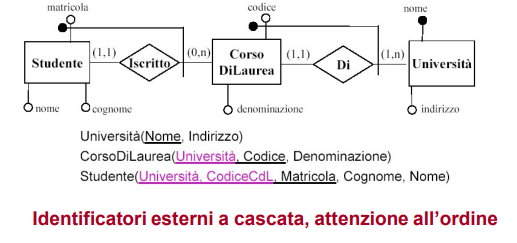
\includegraphics[width=0.5\textwidth]{identificatori_esterni_a_cascata}
    \caption{identificatori esterni a cascata}
    \label{fig:id-esterni-cascata}
\end{figure}
\subsection{Relazioni uno a uno}
In questo caso si accorpa la relazione in un'entità, si sceglie di solito quella con con cardinalità 1-1 dato
che nel caso 0-1 la partecipazione alla relazione è opzionale e quindi si avrebbe un valore NULL.\\
Nel caso di relazioni dove entrambe le entità hanno cardinalità 0-1 si può introdurre una relazione aggiuntiva, 
in modo tale da rappresentare la partecipazione opzionale in entrambi i casi, senza avere valori nulli
sugli attributi (però si introduce una relazione in più). Oppure indicare che le chiavi esterne e gli attributi
della relazioni possono essere nulli.
\section{Documentazione deli schemi logici}
Si devono documentare i vincoli di integrità referenziale, in modo tale da produrre un diagramma con
collegamenti fra relazioni (utili anche per visualizzare i cammini di join).


\chapter{SQL - Structured Query Language}
SQL è un linguaggio per la definizione e la manipolazione dei dati
in database relazionali adottato da molti DBMS. \\
Ci sono diverse versioni, la prima versione ufficiale risale al 1986.
Poi sono state rilasciate altre versioni come SQL-89, SQL-2, SQL-3\dots\\
Noi faremo riferimento principalmente a SQL-2. Questa versione è ricca e complessa,
tanto che nessun sistema commerciale lo implementa in maniera completa.\\
Esistono 3 livelli di conformità:
\begin{itemize}
  \item Entry level: molto simile a SQL-89
  \item Intermediate level: versione che soddisfa le esigenze di mercato
  \item Full level: versione completa anche delle funzioni avanzate che non sono realizzate
        in alcun DBMS
\end{itemize}
La maggior parte dei database è conforme solo all'entry level.\\
Alcune famose implementazioni di SQL sono:
\begin{itemize}
  \item ORACLE
  \item DB2 (IBM)
  \item Access (Microsoft)
  \item MSSQL server (Microsoft)
  \item MySQL
  \item Firebird
\end{itemize}
\section{Confronto con Algebra Relazionale e Istruzioni principali}
\subsection{SQL e Algebra Relazionale}
SQL è relazionalmente completo: ogni espressione logica può essere tradotta in SQL.
Viene adottata la logica dei 3 valori (T, F, U) dell'Algebra relazionale (U = Unknown).\\
Il modello dati di SQL è basato su tabelle anzichè relazioni (possono essere presenti righe duplicate).\\
SQL è computazionalmente completo, ha istruzioni di controllo.\\
\paragraph*{Logica a 3 valori} Logica che utilizza:
\begin{itemize}
  \item True
  \item False
  \item Unknown
\end{itemize}
Che segue la seguente tabella di verità
\begin{table}[h]
  \centering
  \caption{SQL Three-Value Logic Truth Table}
  \begin{tabular}{|c|c|c|c|}
    \hline
    \textbf{Value 1} & \textbf{Value 2} & \textbf{AND} & \textbf{OR} \\
    \hline
    TRUE             & TRUE             & TRUE         & TRUE        \\
    \hline
    TRUE             & FALSE            & FALSE        & TRUE        \\
    \hline
    TRUE             & UNKNOWN          & UNKNOWN      & TRUE        \\
    \hline
    FALSE            & TRUE             & FALSE        & TRUE        \\
    \hline
    FALSE            & FALSE            & FALSE        & FALSE       \\
    \hline
    FALSE            & UNKNOWN          & FALSE        & UNKNOWN     \\
    \hline
    UNKNOWN          & TRUE             & UNKNOWN      & TRUE        \\
    \hline
    UNKNOWN          & FALSE            & FALSE        & UNKNOWN     \\
    \hline
    UNKNOWN          & UNKNOWN          & UNKNOWN      & UNKNOWN     \\
    \hline
  \end{tabular}
\end{table}

\subsection{Istruzioni principali DDL}
Operazioni di definizione schema e modifica
\begin{itemize}
  \item CREATE - Definisce database, tabelle, domini, viste, vincoli e autorizzazioni
  \item ALTER - Modifica attributi e vincoli
  \item DROP - Elimina database e tabelle
\end{itemize}
\subsection{Istruzioni principali DML}
Operazione di interrogazione: SELECT. Formula Query come nell'AR o anche
richieste più elaborate.\\
\subsection*{Aggiornamento}
\begin{itemize}
  \item INSERT - Inserisce nuove tuple nelle tabelle
  \item DELETE - Elmina tuple nelle tabelle
  \item UPDATE - Modifica tuple
\end{itemize}
Queste ultime possono basarsi sul risultato di una query.
\subsection{SQL è dichiarativo}
Essendo principalmente dichiarativo non possiamo scegliere l'ordine in cui
avvengono le operazioni è necessario attenersi alla struttura sintattica delle
istruzioni.
\subsection{Notazione SQL}
\begin{itemize}
  \item Termini del linguaggio in MAIUSCOLO
  \item Termini variabili (specificati dall'utente) in minuscolo
  \item <x> usate per isolare un termine x
  \item [x] indicano che il parametro è opzionale
  \item | seprara opzioni alternative
\end{itemize}

\subsection{Primo esempio di Query}
\begin{lstlisting}[language=SQL]
  SELECT ListaAttributi
  FROM ListaTabelle
  [WHERE Condizione]
\end{lstlisting}
Dove SELECT e FROM sono obbligatori, mentre WHERE è opzionale (in realtà c'è praticamente
sempre in quanto serve per filtrare i risultati).\\
\section{SQL-DDL}
Uno schema di base di dati è una collezione di oggetti: domini, tabelle,
asserzioni, viste, privilegi. La sintassi è la seguente:
\begin{lstlisting}[language=SQL]
  CREATE SCHEMA 
    [Nome Schema]
    [[AUTHORIZATION] Autorizzazione]
    {DefinizioneElementoSchema}
\end{lstlisting}
Nome schema se omesso indica l'utente che ha lanciato il comando, mentre
autorizzazione è il proprietrio dello schema (utente che lo ha definito).\\
\subsection{Tabelle}
Tramite CREATE TABLE si definisce una tabella. Una tabella non è altro che uno
schema di relazione, con CREATE viene creata un'istanza vuota.
\begin{lstlisting}[language=SQL]
  CREATE TABLE NomeTabella
    (NomeAttributo1 TipoDominio1 [Valore di Default] [Vincolo1],
    NomeAttributo2 TipoDominio2 [Valore di Default] [Vincolo2],
    ...
    [AltriVincoli])
\end{lstlisting}
In questo ambito parleremo di tabelle e non di relazioni, e di righe e non di tuple,
perchè rispetto al modello relazionale possiamo avere righe duplicate.\\
Qui di seguito un esempio reale di definizione di tabella:
\begin{lstlisting}[language=SQL]
  CREATE TABLE Impiegato(
    Matricola CHAR(6) PRIMARY KEY,
    Nome CHAR(20) NOT NULL,
    Cognome CHAR(20) NOT NULL,
    Dipart CHAR(15),
    Stipendio NUMERIC(9) DEFAULT 0,
    FOREIGN KEY(Dipart) REFERENCES
    Dipartimento(NomeDip),
    UNIQUE (Cognome,Nome)
)
\end{lstlisting}
\subsection{Definizione dei Dati: I Domini}
I domini specificano i vlori ammessi da ciascun attributo. SQL ha 
6 domini elementari predefiniti:
\begin{itemize}
  \item Carattere- VARCHAR - Stringa di lunghezza variabile tra 0 e n
  \item Numerico Esatto - INTEGER, SMALLINT, NUMERIC
  \item Numerico Approssimato - FLOAT, REAL, DOUBLE PRECISION
  \item Data/Ora TIMESTAMP, DATE, TIME
  \item Intervallo Temporale
  \item Bit (SQL-2) - BOOLEAN (SQL-3) - con dominio 0,1
\end{itemize}
Bit è stato poi eliminato e sostituito parzialmente da BOOLEAN in SQL-3\\
L'utente pu definire dei domini custom (semplici, ma riutilizzabili).\\
\paragraph*{BLOB, CLOB} sono oggetti di grandi dimensioni, costituiti da binari (BLOB)
o caratteri (CLOB), vengono memorizzati in maniera differente dagli altri dati e sono usati per memorizzare
informazioni non strutturate (immagini, video, testi\dots).\\
\subsection{Il tipo Bit}
Utilizzato spesso per definire se è presente o meno una certa proprietà, dato
che si tratta di un BOOLEAN.
\subsection{Carattere}
Si indica:
\begin{lstlisting}[language=SQL]
  CHAR(n) - Stringa di lunghezza fissa n
  VARCHAR(n) - Stringa di lunghezza variabile tra 0 e n
\end{lstlisting}
\subsection{Numerici Esatti}
Rappresentano numeri interi o numeri decimali in virgola fissa (con un numero prefissato
di decimali, come per i valori monetari). Precisionè il numero di cifre significative,
scala il numero di cifre dopo la virgola.\\
\begin{itemize}
  \item INTEGER/SMALLINT rappresentano valori interi - La precisione varia a seconda della
  specifica implementazione di SQL, SMALLINT richiede meno spazio di memorizzazione
  \item NUMERIC/DECIMAL rappresentano valori decimali - La differenza fra questi due è che
  il primo deve essere implementato esattamente con la precisione richiesta, mentre il secondo
  può avere una precisione maggiore.
\end{itemize}
\subsection{Numerici Approssimati}
Sono utili per rappresentare valori reali approssimati, ad esempio grandezze
fisiche (rappresentazione in virgola mobile, in cui a ciascun numero corrisponde
una coppia di valori: mantissa e esponente).\\
REAL e DOUBLE PRECISION rappresentano valori a singola/doppia precisione in virgola
mobile. FLOAT permette di richiedere la precisione che si desidera.
\subsection{Data e Ora}
Permettono di descrivere informazioni temporali, rappresentando istanti di tempo:
\begin{itemize}
  \item DATE rappresenta le date espresse come anno (4 cifre), mese (2 cifre) e giorno (2 cifre)
  - DATE 'yyyy-mm-dd'
  \item TIME [WITH TIME ZONE] rappresenta l'ora del giorno, espressa come ora (2 cifre), 
  minuti (2 cifre) e secondi (2 cifre)
  \item TIMESTAMP
\end{itemize}
Ciascuno di questi domini è strutturato e decomponibile in un insieme di campi 
(anno, mese, giorno, ora, minuti, secondi).
\subsection{Intervalli temporali}
Permette di rappresentare intervalli di tempo come durate di eventi.\\
INTERVAL rappresenta una durata temporale, esistono interval ani e mesi, oppure
giorni e ore, ma non mesi e giorni poichè i mesi non hanno tutti lo stesso numero di
giorni.
\subsection{CLOB e BLOB}
Permettono di includere nel database oggetti molto grandi (come dati multimediali).
Sono implementati come valore e non possono essere usati come criterio di selezione per le
query.
\subsection{Domini definiti dall'utente}
\begin{lstlisting}[language=SQL]
  CREATE DOMAIN Voto AS SMALLINT
    DEFAULT 0
    CHECK (VALUE >= 18 AND VALUE <= 30)
\end{lstlisting}
Possono mettere vincoli puù o meno utili.\\
Al contrario dei meccanismi di definizione dei tipi nei linguaggi di programmazione,
SQL-2 non mette a disposizione dei costruttori di dominio come record o array. Questa 
caratteristica deriva dal modello relazionale dei dati il quale richiede che ogni
attributo sia definito su un dominio elementare.
\subsection{Valori di Deafult}
Definiscono il valore che deve assumere l'attributo quando non viene specificato 
un valore durante l'inserimento di una tupla.\\
DEFAULT $<$ ValoreGenerico | user | null $>$
\begin{itemize}
  \item ValoreGenerico rappresenta un valore compatibile con il dominio,
  rappresentato come una costante o come un’espressione.
  \item user è l’identificativo dell’utente che effettua il comando di
  aggiornamento della tabella.
  \item null è il valore di DEFAULT di base.
\end{itemize}
\subsection{Il valore NULL}
\'E un valore polimorfico che appartiene a tutti i domini con il significato di valore
non noto.
\begin{itemize}
  \item Il valore esiste ma non è noto al database
  \item Il valore è inapplicabile (es. numero patente per minorenni)
  \item Non si sa se il valore è inapplicabile o meno (es. numero patente per un maggiorenne)
\end{itemize}
\subsection{Vincoli di Integrità}
Un vincolo è una regola che specifica delle condizioni sui valori di un elemento
dello schema del database. Un vincolo può essere associato ad una tabella, ad un attributo,
ad un dominio.
\begin{itemize}
  \item Vincoli Intrarelazionali - Proprietà sempre valida all'interno di una relazione
  \item Vincoli Interrelazionali - Proprietà sempre valida tra relazioni diverse
\end{itemize}
\paragraph*{Sintassi}
\begin{itemize}
  \item NOT NULL - Valore non nullo
  \item UNIQUE - Valore unico
  \item PRIMARY KEY - Chiave primaria
  \item CHECK - Definisce condizioni complesse (sia intra che inter relazionali)
\end{itemize}
\paragraph*{Esempio}
\begin{lstlisting}[language=SQL]
  Nome CHAR(20) NOT NULL
  Cognome CHAR(20) NOT NULL 
  UNIQUE (Nome, Cognome)
\end{lstlisting}
NOT NULL su Nome e Cognome è un vincolo intrarelazionale,
UNIQUE è Interrelazionale (non posso avere istanze uguali ripetute)
\subsection{Chiave}
Insieme di attributi che identificano univocamente una tupla all'interno di
una relazione. Il vincolo PRIMARY KEY può essere definito una volta sola all'interno
della relazione (implicitamente NOT NULL e UNIQUE).
\paragraph*{Eccezioni} Il valore NULL può comparire su diverse righe senza violare
il vincolo.
\subsection*{CHECK e FOREING KEY}
Utilizzato per definire vincoli complessi, sia intrarelazionali che interrelazionali.
\begin{lstlisting}[language=SQL]
  CREATE TABLE Studente (
    CREATE DOMAIN Voto AS SMALLINT
    DEFAULT 0
    CHECK (Voto>=18 AND VOTO<=30)
  )
\end{lstlisting}
Per quanto riguarda invece i vincoli interrelazionali, si utilizza FOREIGN KEY e
REFERENCES.\\
\paragraph*{FOREIGN KEY} Un vincolo di intergrità referenziale ("FOREIGN KEY") 
fra gli attributi X di una relazione $R_1$ e un'altra relazione $R_2$ impone ai valori su X,
in $R_1$ di comparire come vlaori della chiave primaria di $R_2$.\\
Un vincolo di intergrità referenzialie fra gli attributi $X={A_1, A_2,...}$ di una
tabella figlio interna e un'altra tabella padre esterna impone ai valori degli attributi X
nella tabella Figlio di comparire come valori della chiave primaria nella Tabella Padre.\\
Alcuni attributi della tabella figlio sono definiti come FOREIGN KEY e si devono riferire (REFERENCES)
ad alcuni attributi della tabella padre che costituiscono una chiave (devono essere UNIQUE e NOT NULL, oppure
PRIMARY KEY).\\
I valori contenuti nella FOREIGN KEY devono essere sempre presenti nella tabella
padre.\\
La tabella Figlio viene anche definita \textbf{interna}, mentre quella Padre \textbf{esterna}.\\
\paragraph*{Due sintassi} 
\begin{enumerate}
  \item Nella parte di definizione degli attributi con il costrutto sintattico
  REFERENCES
  \begin{lstlisting}
    AttrFiglio CHAR(3) REFERENCES TabellaPadre(AttrPadre)
  \end{lstlisting}
  \item Oppure dopo le definizione degli attributi con i costrutti FOREIGN KEY e REFERENCES
  \begin{lstlisting}
    FOREIGN KEY (AttrFiglio) REFERENCES TabellaPadre(AttrPadre)
  \end{lstlisting}
\end{enumerate}
Quando si hanno più attributi da riferire si utilizza sempre FOREIGN KEY e REFERENCES, se si
omettono gli attributi destinazione, vengono assunti quelli della chiave primaria.
\subsection{Aggiornamenti e Violazioni}
Se viene eseguita un'operazione di aggiornamento che viola un vincolo di integrità referenziale
la base di dati diventa non valida, per questo sono definite un insieme di politiche
per evitare che questo accada. Per i vincoli di integrità SQL permette di
scegliere delle reazioni da adottare in caso di violazioni, tali politiche vanno
dichiarate nella dichiarazione DDL dello schema.\\
Si possono introdurre violazioni operando sulle righe della tabella padre (esterna) o sulle righe
della tabella efiglio (interna)
\paragraph*{Modifiche Tabella Figlio}
\begin{itemize}
  \item Inserimento nuova riga
  \item Modifica della FOREIGN KEY
\end{itemize}
Non venogno proposte delle reazioni, le operazioni vengono rifiutate
\paragraph*{Tabella Padre}
\begin{itemize}
  \item Cancellazione riga
  \item Modifica dell'attributo riferito
\end{itemize}
Vengono proposte diverse reazioni:
\begin{itemize}
  \item CASCADE - L'operazione modifica/cancellazione viene propagata alla tabella figlio (o tabella interna)
  \item SET NULL - NULL nella tabella figlio in entrambi i casi
  \item SET DEFAULT - default nella tabella figlio in entrambi i casi
  \item NO ACTION - rifiutata in entrambi i casi
\end{itemize}
Le politiche di reazione possono essere definite in modo diverso per eventi di modifica/cancellazione
\begin{lstlisting}[language=SQL]
  Dipart CHARACTER(15) REFERENCES Dipartimento(NomeDip)
    ON DELETE SET NULL
    ON UPDATE CASCADE
\end{lstlisting}
Con CASCADE in pratica se effettuo una cancellazione cancello anche tutte le relazioni legati a quel valore,
con NULL invece pongo a NULL la FOREIGN KEY, ma mentengo gli altri valori.
\'E possibile assegnare un nome a questi vincoli, per rendere più chiaro il codice e rendere
quindi più semplice il debugging e la scrittura della documentazione.
\paragraph*{Sintassi nome vincoli}
\begin{lstlisting}[language=SQL]
  Stipendio INTEGER CONSTRAINT StipendioPositivo
  CHECK (Stipendio > 0),
  ...
  CONSTRAINT ForeignKeySedi
  FOREIGN KEY (Sede) REFERENCES Sedi
\end{lstlisting}

\section{Modifiche degli schemi}
Necessarie per garantire l'evoluzione della base di dati a fronte di nuove esigenze.\\
Ci sono 2 comandi SQL appositi:
\begin{itemize}
  \item ALTER - Modifica oggetti
  \item DROP - Cancella oggetti dallo schema
\end{itemize}
\subsection{ALTER}
\begin{itemize}
  \item ALTER DOMAIN - modifica domini (default, vincoli)
  \item ALTER TABLE - modifica tabelle
\end{itemize}
Attenzione: Quando si definisce un nuovo vincolo deve essere soddisfatto dalla istanza 
presente, altrimenti viene rifiutato.
\paragraph*{Modifiche degli schemi - DROP}
\begin{itemize}
  \item DROP DOMAIN - cancellazione del dominio (attributo)
  \item DROP TABLE - cancellazione della tabella
\end{itemize}
\paragraph*{Opzioni}
\begin{itemize}
  \item RESTRICT - Un oggetto (dominio, tabella) non è rimosso se non è vuoto
  \item CASCADE - viene rimosso l'oggetto e tutto ciò che è coinvolto
  nella definizione dell'oggetto
\end{itemize}
\paragraph*{Sintassi ALTER}
\begin{lstlisting}[language=SQL]
  ALTER DOMAIN NomeDominio <
    SET DEFAULT ValoreDefault|
    DROP DEFAULT|
    ADD CONSTRAINT DefVincolo |
    DROP CONSTRAINT NomeVincolo >
\end{lstlisting}
Esempio ALTER su tabella
\begin{lstlisting}[language=SQL]
  ALTER TABLE NomeTabella <
    ALTER COLUMN NomeAttributo<
      SET DEFAULTNuovoDefault |
      DROP DEFAULT> |
    DROP COLUMN NomeAttributo |
    ADD COLUMN DefAttributo |
    DROP CONSTRAINTNomeVincolo
    ADD CONSTRAINTDefVincolo >
\end{lstlisting}
\paragraph*{Sintassi DROP}
\begin{lstlisting}[language=SQL]
  DROP <schema, domain, table, view, ...> NomeElemento
    [RESTRICT | CASCADE]
\end{lstlisting}
\begin{itemize}
  \item RESTRICT - Impedisce drop se gli oggetti comprendono istanze non vuote
  \item CASCADE - Applica drop agli oggetti collegati, Potenziale pericolosa reazione
  a catena
\end{itemize}
\subsection{Cataloghi relazionali}
Il catalogo contiene il dizionario dei dati (data dictionary) ovvero la descrizione
della struttura dei dati contenuti nel database. Anche questa descrizione di dati (metadati)
è rappresentata tramite una struttura relazionale.\\
SQL-2 Organizza il catalogo su due livelli:
\begin{itemize}
  \item Definition\_Schema (composto da tabelle che descrivono tutte le strutture della
  base di dati)
  \item Information\_Schema (composto da viste che costituiscono l'interfaccia verso 
  il dizionario dei dati)
\end{itemize}

\section{Interrogazioni SQL - Query}
Le interrogazioni avvengono usando l'istruzione SELECT
\begin{lstlisting}[language=SQL]
  SELECT ListaAttributi
  FROM ListaTabelle
  [ WHERE Condizione ]
\end{lstlisting}
\begin{itemize}
  \item SELECT indica quali attributi vogliamo nel risultato
  \item FROM indica le tabelle da cui estrarre i dati
  \item WHERE indica che condizioni devono essere soddisfatte
\end{itemize}
SELECT non significa selezione, sceglie le colonne output della query.\\
FROM se vengono indicate più tabelle si effettua il loro prodotto cartesiano, 
salvo diversamente specificato (es. JOIN).\\
\subsection{Istruzione AS}
Si possono fare ridenominazioni su attributi e anche su relazioni con la clausola AS, 
molto utile per evitare di scrivere ogni volta l'attributo o la tabella per esteso
(specialmente se i nomi sono lunghi).\\
\begin{lstlisting}[language=SQL]
  SELECT AttrEspr [[AS] Alias]{,AttrEspr [[AS] Alias]}
  FROM Tabella [[AS] Alias]{,Tabella [[AS] Alias]}
  [WHERE Condizione]
\end{lstlisting}
Esempio pratico:
\begin{lstlisting}[language=SQL]
  SELECT Nome AS N, Stipendio AS Salario
  FROM Dipendente AS Dip
  WHERE Dip.Stipendio > 1000
\end{lstlisting}
\subsection{Asterisco}
Per selezionare tutti gli attributi viene utilizzato *.
\subsection{FROM clausola .}
La clausola PUNTO . permette di specificare a che relazione
appartiene un attributo (o anche una tabella o un database).\\
Esempio:
\begin{lstlisting}[language=SQL]
  SELECT Dip.Nome, Dip.Stipendio
  FROM Dipendente AS Dip
  WHERE Dip.Stipendio > 1000
\end{lstlisting}
Si possono ovviamente usare gli alias denominati con AS dato che
viene prima letta la parte del FROM.\\
\subsection{WHERE}
Parte fondamentale della Query (seppur opzionale), specifica la
condizione di selezione. L'argomento do WHERE è un'espressione booleana:\\
\begin{lstlisting}[language=SQL]
  WHERE [NOT] PredicatoSemplice {< AND | OR > [NOT] PredicatoSemplice}
\end{lstlisting}
\paragraph*{Operatori di confronto}
\begin{itemize}
  \item =, <>, !=, >, >=, <, <=
  \item BETWEEN valore1 AND valore2
  \item IN (valore1, valore2, ...)
  \item LIKE 'stringa' (con \% e \_ per sostituire caratteri)
  \item IS NULL, IS NOT NULL
\end{itemize}
Si selezionano per il risultato solo le tuple per le quali l'espressione
che segue la clausola WHERE è vera.\\
\paragraph*{Precedenza operatori Booleani}
\begin{itemize}
  \item NOT
  \item AND
  \item OR
\end{itemize}
Per stabilire la precedenza \textbf{usare sempre le parentesi}.\\
\subsection{WHERE - Operatore Like}
L'operatore LIKE permette di esprimere dei pattern su stringhe di
caratteri mediante la seguente notazione:
\begin{itemize}
  \item \_ indica un singolo carattere arbitrario
  \item \% indica una stringa di caratteri arbitraria (anche lunga 0)
\end{itemize}
\paragraph*{Esempio} Tutti nomi degli impiegati che finiscono con una i
e hanno una 0 in seconda posizione:
\begin{lstlisting}[language=SQL]
  SELECT Nome
  FROM Impiegato
  WHERE Nome LIKE '_o%i'
\end{lstlisting}
\subsection{WHERE - Operatore BETWEEN}
L'operatore BETWEEN permette di esprimere condizioni di appartenenza
a un intervallo.
\begin{lstlisting}[language=SQL]
  WHERE Attributo BETWEEN Valore1 AND Valore2
\end{lstlisting}
\subsection{WHERE - Operatore IN}
L'operatore IN permette di esprimere condizioni di appartenenza 
a un insieme.
\paragraph*{Esempio} Cognome e numero uffcio degl impiegati negli
uffici 10 e 20:
\begin{lstlisting}[language=SQL]
  SELECT Cognome, ufficio
  FRM Impiegato
  WHERE ufficio IN ('10', '20')
\end{lstlisting}
Si poteva anche usare:
\begin{lstlisting}[language=SQL]
  WHERE ufficio = '10' OR ufficio = '20'
\end{lstlisting}
\subsection{WHERE - Valori nulli}
SQL-2 usa una logica a tre valori per valutare il valore di verità
di una clausola WHERE: True (T), Flase (F), Unkown (?).\\
Un predicato semplice valutato su un attributo a valore nullo dà come
risultato della valutazione ?.\\
Una tupla per cui il valore di verità è ? non viene restituita dalla query.\\
Se la valutazione del predcato di un constraint è ? il constraint non
è violato.\\
\paragraph*{Tabella di verità}
\begin{figure}[h]
  \centering
  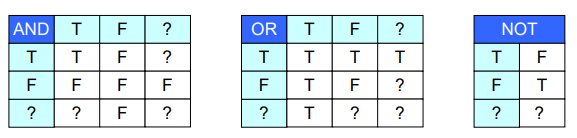
\includegraphics[width=0.7\textwidth]{tabella_verit_sql.png}
  \caption{Tabella di verità}
  \label{fig:tabella_verita-SQL}
\end{figure}
Per valutare gli attributi nulli è necessario usare IS NULL o IS NOT NULL.\\
\begin{itemize}
  \item IS NULL - vero se attributo ha valore nullo, falso altrimenti
  \item IS NOT NULL - vero se attributo ha valore specificato, falso altrimenti
\end{itemize}
\paragraph*{Esempio per la seguente tabella}
\begin{tabular}{|c|c|c|}
  \hline
  A & B & C \\
  \hline
  a & ? & c1 \\
  \hline
  a1 & b & c2 \\
  \hline
  a2 & ? & ? \\
  \hline
\end{tabular}
\begin{lstlisting}[language=SQL]
  SELECT *
  FROM Tabella
  WHERE B IS NULL
\end{lstlisting}
Restituisce t1 e t3.
\paragraph*{Esempio reali} Query: gli impiegati che \textbf{sono} o \textbf{potrebbero essere}
ingegneri.
\begin{lstlisting}[language=SQL]
  SELECT *
  FROM Impiegato
  WHERE mansione = 'Ingegnere' OR mansione IS NULL
\end{lstlisting}
\subsection{SELECT - DISTINCT}
In algebra relazionale i risultati della interrogazioni non contengono
elementi duplicati, mentre in SQL le tabelle prodotte dalle interrogazioni
possono contenere più righe identiche tra loro.\\
I duplicati possono essere rimossi usando la parola chiave DISTINCT.
\begin{lstlisting}[language=SQL]
  SELECT [DISTINCT] AttrEspr
  FROM Tabella
  [WHERE Condizione]
\end{lstlisting}
\subsection{Espressioni e Funzioni}
I predicati usati nelle interrogazioni possono coinvolgere, oltre a
nomi di colonna anche espressioni. Le espressioni sono formulate
applicando operatori ai valori delle colonne delle tuple.\\
Esempi di espressioni e funzioni sono que40lle aritmetiche su stringhe,
su date e tempi. Le espressioni possono comparire nelle clausole
SELECT, WHERE e UPDATE.
\paragraph*{SELECT} Una espressione usata nella clausola SELECT
dà luogo ad una nuova colonna che non corrisponde a nessuna colonna
della tabella su cui si effettua la selezione (argomento di FROM).\\
Questa colonna è detta Colonna \textbf{virtuale}. Le colonne virtuali non sono
fisicamente memorizzate, ma sono materializzate (esistono) solo come risultato
delle interrogazioni.\\
Anche alle colonne virtuali è possibile assegnare un alias (con il
costrutto AS).\\
\paragraph*{Funzioni predefinite}
\begin{itemize}
  \item su stringhe (UPPER, UCASE, LENGTH)
  \item su date, intervalli (+, -, DATE, DAYOFWEEK, ...)
  \item matematiche (*, +, -, /, TAN, SQRT, SIN, ...)
  \item informazioni di istema (USER, CURRENT\_DATE, ...) 
\end{itemize}
\paragraph*{Esempio} Trovare stipendio mensile degli impiegati che guadagnano
più di 40.\\
Dato che lo stipendio memorizzato nel DB è annuale, bisogna dividere per 12.
\begin{lstlisting}[language=SQL]
  SELECT stipendio/12 AS stipendio_mensile
  FROM Impiegato
  WHERE stipendio > 40
\end{lstlisting}
Se non inserisco un ALIAS la colonna virtuale avrà un nome generato (non significativo).
\paragraph*{Funzioni per le stringhe}
Gli operatori più comuni sono:
\begin{itemize}
  \item || - concatenazione
  \item UPPER, UCASE - Trasforma la stringa in caratteri maiuscoli
  \item LOWER, LCASE - Trasforma la stringa in caratteri minuscoli
\end{itemize}
\section{Operatore JOIN}
L'operatore JOIN rappresenta un'importante funzionalità in quanto
permette di correlare dati in tabelle diverse.\\
Matematicamente si tratta del prodotto cartesiano tra le due tabelle,
che avrà un numero di righe pari al prodotto del numero di righe
delle due tabelle e viene applicata una condizione di matching tra 
le colonne specificate. Il puro prodotto cartesiano avviene fra le
tabelle inserite nel FROM, mentre la condizione di matching è inserita
o nel WHERE (\textbf{JOIN implicito}) o nel FROM esplicitando il JOIN (\textbf{JOIN esplicito}).\\
Ad un operatore JOIN sono applicati uno o più predicati di join.\\
Un predicato di join esprime una condizione che deve essere verificata
dalle tuple del risultato dell'interrogazione.
Il predicat di join permette di estrarre dal DB un sottoninsieme opportuno
del prodotto cartesiano.
\subsection{JOIN implicito}
Quando la condizione di selezione viene inserita nel WHERE allora sto
effettuando un JOIN implicito.
\paragraph*{Esempio}
\begin{lstlisting}[language=SQL]
  SELECT *
  FROM Impiegato, Dip
  WHERE Impiegato.Dipart = Dip.Nome;
\end{lstlisting}
In questo caso ho estratto tutte le informazioni sugli impiegati e sui
dipartimenti in cui lavorano.\\
\paragraph*{Esempio Esami}
Estrarre Matricola, Cognome, Nome Voto di tutti gli studenti che
hanno sostenuto l'esame di 'Analisi I'.
\begin{lstlisting}[language=SQL]
  SELECT S.Matricola, S.Cognome, S.nome, E.Voto
  FROM Studenti AS S, Esami AS E
  WHERE (S.Matricola = E.Studente) AND (E.Corso = 'Analisi I')
\end{lstlisting}
Come già detto in precedenza il FROM efettua il prodotto cartesiano, mentre
la condizione di WHERE indica il predicato di join.\\
\subsection{JOIN esplicito}
Introdotto in SQL-2, è possibile effettuare esplicitamente il JOIN
nella clausola FROM
\begin{lstlisting}[language=SQL]
  SELECT AttrExpr [ [AS] Alias ] {, AttrExpr [[AS] Alias ] }
  FROM Tabella [ [AS] Alias ]
  { [ TipoJoin ] JOINTabella [[AS] Alias ] ONCondizJoin}
  [ WHERE CondizQuery ]
\end{lstlisting}
In questo modo esplicitiamo il JOIN sulle tabelle e separiamo
le condizioni di JOIN dalle condizioni di QUERY.
\paragraph*{Tipi di JOIN}
\begin{itemize}
  \item INNER (questo prefisso non si mette dato che è il JOIN di default)
  \item OUTER JOIN
  \begin{itemize}
    \item RIGTH [OUTER]
    \item LEFT [OUTER]
    \item FULL [OUTER]
  \end{itemize}
\end{itemize}
\paragraph*{Esempio JOIN sul seguente schema}
\begin{center}
  \begin{tabular}{|c|c|c|c|c|c|c|c|c|c|}
    \hline
    ID\_impiegato & Nome & Cognome & Dipart & Ufficio & Stipendio & premioprod & Mansione & Città & IDCapo \\
    \hline
  \end{tabular}
\end{center}
\begin{tabular}{|c|c|c|}
  \hline
  Nome & Indirizzo & Città\\
  \hline
\end{tabular}
\begin{lstlisting}[language=SQL]
  SELECT I.Nome, I.Cognome, Dip.Citta
  FROM Impiegato AS I JOIN Dip ON I.Dipart = Dip.Nome
\end{lstlisting}
Non si ha traccia delle tuple di impiegato che non corrispondono
ad alcuna tupla di Dip.
\subsection{OUTER JOIN}
L'operatore di OUTER JOIN aggiunge l risultato le tuple di Impiegato e Dip che non hanno partecipato al JOIN,
completandole con NULL.\\
Consideriamo il seguente esempio:
\begin{lstlisting}[language=SQL]
  FROM Impiegato AS I [FULL|LEFT|RIGHT] OUTER JOIN Dip ON ...
\end{lstlisting}
\paragraph*{LEFT} Le tuple di impiegato che non partecipano al join vengono completate ed inserite
nel risultato.
\paragraph*{RIGHT} Le tuple di Dip che non partecipano al join vengono completate ed inserite nel
risultato.
\paragraph*{FULL} (Sia Left che Right) Sia le tuple di impiegato che quelle di Dip che non partecipano al join
vengono completate ed inserite nel risultato.
\subsection{Self JOIN}
JOIN effettuato sulla stessa tabella.
\paragraph*{Esempio}
\begin{lstlisting}[language=SQL]
  SELECT G1.Genitore AS Nonno
  FROM Genitori G1, Genitori G2
  WHERE G1.Figlio = G2.Genitore
  AND G2.Figlio = 'Anna'
\end{lstlisting}
In questo caso vengono ricercati i nonni di Anna. \'E possibile fare questo perchè
quando seleziono le tabelle nel FROM tratto delle loro copie, quindi posso anche prenderle due volte.
\section{Operatori di ordinamento e aggregazione}
\subsection{Ordinamento del risultato: ORDER BY}
Le righe sono ordinate in base al primo attributo, se i valori sono uguali,
viene ordinata in base al secondo attributo ecc.\\
Ordinamento: ascendente (ASC), discendente (DESC), (ASC è default e può
essere omesso).
\paragraph*{Esempio}
\begin{lstlisting}[language=SQL]
  SELECT *
  FROM Impiegato
  ORDER BY Stipendio
\end{lstlisting}
L'opzione DESC è relativa al singolo attributo, quindi va specificata per ciascun attributo
che elenco nell'ORDER BY.\\
\subsection{Operatori aggregazione}
Sono un'estensione rispetto all'Algebra Relazionale. Essi operano su gruppi di tuple per:
\begin{itemize}
  \item Effettuare calcoli sull'insieme di tuple
  \item Verificare condizioni relative all'insieme di tuple
\end{itemize}
\begin{itemize}
  \item COUNT - Conta numero di tuple di tabella
  \item SUM - Somma valori o espressioni di attributi
  \item MAX - Valore massimo di un attributo di tabella
  \item MIN - Valore minimo di un attributo di tabella
  \item AVG - Valore medio di un attributo di tabella
  \item GROUP BY - Raggruppamento delle tuple in sottogruppi gestiti come estensione
  delle normali interrogazioni
\end{itemize}
\paragraph*{Come vengono applicati}
\begin{itemize}
  \item Si esegue l'interrogazione sulla base di clausole FROM e WHERE.
  \item Si applica l'operatore aggregato alla tabella risultato dell'interrogazione.
\end{itemize}
\subsection{COUNT}
\begin{lstlisting}[language=SQL]
  SELECT COUNT(< * | [DISTINCT | ALL] ListaAttr >)
\end{lstlisting}
\begin{itemize}
  \item DISTINCT numero di valori distinti diversi da NULL di ListaAttr
  \item ALL numero di valori diversi da NULL di ListaAttr
  \item COUNT (*) conta numero di righe di una tabella
\end{itemize}
Se non è specificato nulla, ALL è l'opzione di default.
\paragraph*{Esempio} Estrarre il numero di impiegati del dipartimento Produzione
\begin{lstlisting}[language=SQL]
  SELECT COUNT(*) AS impiegati_produzione
  FROM Impiegato
  WHERE dipart='Produzione'
\end{lstlisting}
L'operatore aggregato COUNT viene applicato al risultato dell'interrogazione.\\
\paragraph*{COUNT e valori nulli}
COUNT(*) conta anche le righe con valori NULL, dato che conta le righe totali della tabella.\\
COUNT(Attributo) non conta le righe NULL.\\
COUNT(DISTINCT Attributo) non conta le righe NULL e non conta i valori duplicati.
\subsection{Altri operatori di aggregazione}
\begin{lstlisting}[language=SQL]
  < SUM | MAX | MIN | AVG > (< * | [DISTINCT | ALL] AttrExpr >)
\end{lstlisting}
Valutano espressioni analizzando tuple del risultato nella query che li contiene. Operano
su tuple di tabella prese come insieme di elementi (non su elementi individuali).
DISTINCT e ALL si applicano come per il caso di COUNT.
\paragraph*{SUM} Restituisce la somma dei valori di AttrExpr relativamente alle tuple di tabella specificate
nella query. Opera su attributi numerici.
\paragraph*{MIN MAX} Restituisce il minimo/massimo dei valori di AttrExpr relativamente alle tuple di tabella 
specificate nella query. Opera su atributi ordinabili (stringhe, numer, ecc.).\\
\paragraph*{AVG} Restituisce la media dei valori di AttrExpr relativamente alle tuple di tabella specificate, opera
su valori numerici.
\subsection{Operatori di aggregazione e Target List}
SQL impedisce di includere in una stessa target list funzioni aggregate e espressioni al livello
di riga.
\paragraph*{Esempio}
\begin{lstlisting}[language=SQL]
  SELECT Cognome, MAX(Stipendio) -- ERRORE
  FROM Impiegato
  WHERE Dipart = 'Amministrazione'
\end{lstlisting}
La soluzione è effettuare una query nidificata (spiegata in seguito).
\begin{lstlisting}[language=SQL]
  SELECT Cognome, Stipendio
  FROM Impiegato
  WHERE Dipart = 'Amministrazione'
  AND Stipendio = (SELECT MAX(I1.Stipendio) 
                  FROM Impiegato AS I1
                  WHERE I1.Dipart = 'Amministrazione')
\end{lstlisting}
\subsection{GROUP BY}
La clausola GROUP BY serve a definire gruppi omogenei di tuple, specificando una o
più colonne (di raggruppamento) sulla base della/e quale/i le tuple sono raggruppate
per valori uguali.\\
\paragraph*{Esempio}
Data la seguente tabella estrarre la somma degli stipendi degli impiegati che afferiscono
allo stesso dipartimento.
\begin{figure}[h]
  \centering
  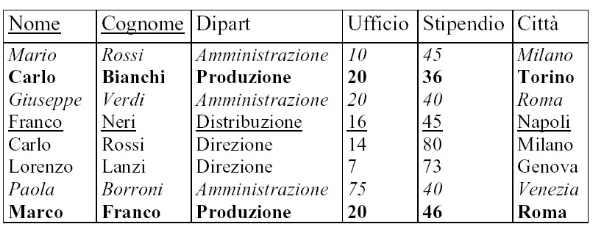
\includegraphics[width=0.7\textwidth]{es_group_by.png}
  \caption{Tabella esercizio}
  \label{fig:tabella_es_groupby}
\end{figure}
\begin{lstlisting}[language=SQL]
  SELECT Dipart, SUM(Stipendio)
  FROM Impiegato
  GROUP BY Dipart
\end{lstlisting}
Come viene eseguita la query? Analizziamola passo per passo:
\paragraph*{Esecuzione senza GROUP BY}
In questo caso mi restituisce tutti gli attributi della SELECT in un'unica tabella.\\
Con GROUP BY invece vengono raggruppate le righe del risultato come specificato
nel GROUP BY (nell'esempio valori Dipart).
\begin{figure}[h]
  \centering
  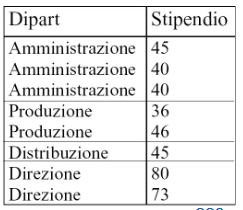
\includegraphics[width=0.3\textwidth]{tabella_groupby.png}
  \caption{Tabella con GROUP BY}
  \label{fig:tabella_groupby}
\end{figure}
\paragraph*{Applicazione SUM dopo GROUP BY} 
Così facendo l'applicazione dell'operatore SUM avviene su gruppi di tuple con lo stesso nome.
\begin{table}[h]
  \centering
  \begin{tabular}{|c|c|}
    \hline
    Dipart & sum(Stipendio) \\
    \hline
    Amministrazione & 125 \\
    \hline
    Produzione & 82 \\
    \hline
    Distribuzione & 45\\
    \hline
    Direzione & 153 \\
    \hline
  \end{tabular}
  \caption{Tabella somma stipendi per dipartimento}
  \label{tabella_stipendi}
\end{table}
\newpage
Il GROUP BY raggruppa sempre gli gli attributi specificati nella clausola GROUP BY con lo stesso
nome, permettendo poi di applicare condizioni particolari nella SELECT (per esempio AVG, COUNT, ecc.).
\subsection{Raggruppamenti e Target List}
\paragraph*{Importante restrizione} Una clausola di proiezione di una query contenente la clausola
GROUP BY può solo includere:
\begin{enumerate}
  \item Una o più colonne se compaiono nella clausola GROUP BY
  \item Operatori di aggregazione (COUNT, SUM, AVG, ...)
\end{enumerate}
Nella SELECT deve apparire l'attributo specificato nel GROUP BY, altrimenti la Query risulterà
scorretta.
\begin{lstlisting}[language=SQL]
  SELECT nome, cognome -- nome e' ERRORE!
  FROM persone
  GROUP BY cognome

  SELECT cognome, AVG(Eta) -- Corretta
  FROM persone
  GROUP BY cognome
\end{lstlisting}
Tutti gli attributi nella SELECT devono essere sepcificati anche nel GROUP BY.
\subsection{Condizioni sui Gruppi}
Verificano condizioni su gruppi di tuple aggregate con GROUP BY.
\begin{itemize}
  \item WHERE - Verifica condizioni su tuple individuali
  \item HAVING - Verifica condizioni (espressioni booleane) su gruppi di tuple
  (opera su raggruppamenti)
\end{itemize}
Le condizioni in clausola HAVING sono verificate dopo la creazione dei sottogruppi
di tuple specificati da GROUP BY.\\
\paragraph*{Esempio}
Trovare i dipartimenti che spendono più di 100 in stipendi.
\begin{lstlisting}[language=SQL]
  SELECT Dipart, SUM(Stipendio) AS SommaStipendi
  FROM Impiegato
  GROUP BY Dipart
  HAVING SommaStipendi > 100
\end{lstlisting}
\paragraph*{Risolviamo la Query passo per passo.}
\begin{enumerate}
  \item Esecuzione della query senza considerare GROUP BY e operatori
  aggregati
  \item Raggruppamento delle righe del risultato come specificato da GROUP BY
  \item Applicazione dell'operatore di aggregazione SUM su Stipendio ai gruppi di
  righe precedentemente costruiti
  \item Selezione dei gruppi risultanti come specificato dalla clausola HAVING
\end{enumerate}
Qui vediamo proprio la differenza di HAVING rispetto a WHERE, dato che
WHERE opera su tuple individuali (selezione di tuple prima di GROUP BY),
mentre HAVING opera su predicati che operano su gruppi di tuple creati da
GROUP BY (selezone raggruppamenti).
\paragraph*{Esempio molto utile} Andare alla slide N 247 (62 come Pagina PDF)
delle slide del prof \href{https://elearning.unimib.it/pluginfile.php/1533829/mod_resource/content/1/SQL.pdf}{Slide Prof}.
\subsection{Osservazioni}
\begin{lstlisting}[language=SQL]
  GROUP BY attr1, attr2
  -- Equivalente a
  GROUP BY attr2, attr1
\end{lstlisting}
\paragraph*{HAVING osservazioni}
La sintassi permette di definire la clausola HAVING anche senza la clausola GROUP BY.
In questo caso l'intero insieme di righe è trattato come un unico raggruppamento, è
necessario ricordarsi che per HAVING devono essere usati solo predicati in cui
compaiono operatori aggregati.
\section{Interrogazioni di tipo insiemistico}
Permettono di costruire query concatenando due query SQL
\begin{itemize}
  \item UNION
  \item INTERSECT
  \item EXCEPT (differenza)
\end{itemize}
\paragraph*{Sintassi}
\begin{lstlisting}[language=SQL]
  SelectSQL { < UNION/INTERSECT/EXCEPT > [ALL] SelectSQL }
\end{lstlisting}
I duplicati vengono eliminati (a meno che si usi ALL).
\subsection{UNION}
Restituisce tutte le tuple distinte restituire da almeno una delle sottointerrogazioni a qui
è applicata.\\
L'operatore UNION elimina i duplicati dal risultato, mentre UNION ALL li mantiene.\\
UNION impone alcune importanti restrizioni sulle interrogazioni su cui opera:
\begin{itemize}
  \item Le interrogazioni devono restituire lo stesso numero di colonne, e le colonne corrispondenti devono avere
  lo stesso dominio (non è richiesto che abbiano la stessa lunghezza) o domini compatibili
  \item La corrispondenza si basa sulla posizione delle colonne, indipendentemente dal loro nome
  \item Se si usa la clausola ORDER BY questa deve essere usata una sola volta alla
  fine dell'interrogazione e non alla fine di ogni SELECT
\end{itemize}
\subsection{INTERSECT, EXCEPT, MINUS}
\begin{itemize}
  \item L'operatore INTERSECT esegue l'intersezione
  \item Gli operatori EXCEPT e MINUS eseguono la differenza
\end{itemize}
Per questi operatori valgono le stesse condizioni di applicabilità viste per l'operatore
UNION. Le interrogazioni devono restituire lo stesso numero di clonne e le colonne corrispondenti
devono avere lo stesso dominio (non è richiesto che abbiano la stessa lunghezza) o domini compatibili.
La corrispondenza si basa sulla posizione delle colonne.\\



\end{document}